\documentclass[aps,prx,twocolumn,superscriptaddress,nofootinbib]{revtex4-2}
\usepackage{amsmath,amssymb,bm}
\usepackage{graphicx}
\usepackage{hyperref}

% Auto-generated by generate_bt2t002_paper_assets.py -- DO NOT EDIT BY HAND
\newcommand{\btmExperimentId}{\texttt{OSIRIS-BT2T-002}}
\newcommand{\btmPaperId}{\texttt{OSIRIS-BT2T-002-PAPER}}
\newcommand{\btmExecTier}{\texttt{SIMULATED}}
\newcommand{\btmCompileTier}{\texttt{OFFLINE\_COMPILED}}
\newcommand{\btmProxyTier}{\texttt{PROXY}}
\newcommand{\btmJobId}{\texttt{null}}
\newcommand{\btmQpuSec}{0}
\newcommand{\btmSeed}{20261124}
\newcommand{\btmEncVer}{\texttt{bt2t-enc-1}}
\newcommand{\btmEncSha}{\texttt{3e3b02d13539daaf}}
\newcommand{\btmManifestSha}{\texttt{e51fb835398eb221}}
\newcommand{\btmMulPySha}{\texttt{00f6fffb5779f15e}}
\newcommand{\btmQftPySha}{\texttt{1296db4fa4013db3}}
\newcommand{\btmVerifyPySha}{\texttt{6d05040123eada74}}
\newcommand{\btmBaseBtPySha}{\texttt{e179cfb1cd431615}}
\newcommand{\btmMoneResSha}{\texttt{4b70cf7210a73ba3}}
\newcommand{\btmStructQasmSha}{\texttt{8f1b3993175de092}}
\newcommand{\btmGenQasmSha}{\texttt{97b3158ea31b359e}}
\newcommand{\btmQftQasmSha}{\texttt{93369014d8cc8170}}
\newcommand{\btmCapsuleSha}{\texttt{d5d5f50cf01d2da3}}
\newcommand{\btmChecksTotal}{31}
\newcommand{\btmChecksPassed}{31}
\newcommand{\btmGroupOrder}{24}
\newcommand{\btmQeightOrder}{8}
\newcommand{\btmZthreeOrder}{3}
\newcommand{\btmRegQubits}{5}
\newcommand{\btmRegStates}{32}
\newcommand{\btmUnusedCodewords}{8}
\newcommand{\btmMulQubits}{10}
\newcommand{\btmMulAncillas}{0}
\newcommand{\btmMulBasisStates}{1,024}
\newcommand{\btmMulBasisStatesRaw}{1024}
\newcommand{\btmValidPairs}{576}
\newcommand{\btmUnusedPairs}{448}
\newcommand{\btmQeightPairs}{64}
\newcommand{\btmNonIdElements}{23}
\newcommand{\btmOmegaIdx}{23}
\newcommand{\btmOmegaSqIdx}{16}
\newcommand{\btmHurwitzCount}{16}
\newcommand{\btmMoneProtocolId}{\texttt{OSIRIS-BT2T-001-FEZ}}
\newcommand{\btmMoneBackend}{\texttt{ibm\_fez}}
\newcommand{\btmMoneJobId}{\texttt{dc2ee3uq4uuc73a56o6g}}
\newcommand{\btmMoneTier}{\texttt{HARDWARE\_ATTESTED}}
\newcommand{\btmMoneWindows}{1}
\newcommand{\btmMoneShots}{27,648}
\newcommand{\btmMoneQpuSec}{11}
\newcommand{\btmMoneAtaStructCz}{48}
\newcommand{\btmMoneAtaGenCz}{400}
\newcommand{\btmMoneAtaRatio}{8.33\times}
\newcommand{\btmMoneFezStructCz}{72}
\newcommand{\btmMoneFezStructSx}{151}
\newcommand{\btmMoneFezStructDepth}{218}
\newcommand{\btmMoneFezGenCz}{723}
\newcommand{\btmMoneFezGenSx}{1,560}
\newcommand{\btmMoneFezGenDepth}{2,073}
\newcommand{\btmMoneFezRatio}{10.04\times}
\newcommand{\btmMoneTkStructZz}{47}
\newcommand{\btmMoneTkGenZz}{400}
\newcommand{\btmMoneTkRatio}{8.51\times}
\newcommand{\btmMonePValidStruct}{0.5337}
\newcommand{\btmMonePValidStructSe}{0.0059}
\newcommand{\btmMonePValidStructMit}{0.6104}
\newcommand{\btmMonePValidGen}{0.0661}
\newcommand{\btmMonePValidGenSe}{0.0030}
\newcommand{\btmMonePValidGenMit}{0.0715}
\newcommand{\btmMoneDeltaValid}{0.4676}
\newcommand{\btmMonePValidCtrl}{0.8643}
\newcommand{\btmMonePUnusedCtrl}{0.9076}
\newcommand{\btmMoneRandFloor}{0.03125}
\newcommand{\btmEsdX}{2}
\newcommand{\btmEsdCx}{6}
\newcommand{\btmEsdCcx}{4}
\newcommand{\btmEsdCswap}{3}
\newcommand{\btmEsdCthreex}{2}
\newcommand{\btmEsdCfourx}{1}
\newcommand{\btmEsdMcxTotal}{3}
\newcommand{\btmEsdTotalGates}{18}
\newcommand{\btmEsdDepth}{15}
\newcommand{\btmEsdOpErr}{0.0}
\newcommand{\btmBarencoLemmaSevenTwo}{7.2}
\newcommand{\btmBarencoLemmaSevenThree}{7.3}
\newcommand{\btmBarencoThreeCcx}{4}
\newcommand{\btmBarencoFourCcx}{8}
\newcommand{\btmBarencoFiveCcx}{12}
\newcommand{\btmBarencoSixCcx}{24}
\newcommand{\btmMulStructCcx}{270}
\newcommand{\btmMulStructCx}{35}
\newcommand{\btmMulStructX}{18}
\newcommand{\btmMulStructCswap}{14}
\newcommand{\btmMulStructMcx}{0}
\newcommand{\btmMulStructTotalGates}{337}
\newcommand{\btmMulStructDepth}{300}
\newcommand{\btmMulGenMcx}{2,040}
\newcommand{\btmMulGenMcxRaw}{2040}
\newcommand{\btmMulGenCx}{1,656}
\newcommand{\btmMulGenX}{1,064}
\newcommand{\btmMulGenCswap}{144}
\newcommand{\btmMulGenTotalGates}{4,904}
\newcommand{\btmMulGenDepth}{3,760}
\newcommand{\btmMulLogGateRatio}{14.55\times}
\newcommand{\btmMulLogDepthRatio}{12.53\times}
\newcommand{\btmMulStructOpErr}{0.0}
\newcommand{\btmMulGenOpErr}{0.0}
\newcommand{\btmMulStructSupErr}{0.0}
\newcommand{\btmMulGenSupErr}{0.0}
\newcommand{\btmMulSupTrials}{32}
\newcommand{\btmMulPhaseCtrlErr}{2.0}
\newcommand{\btmMulAtaStructCz}{1,739}
\newcommand{\btmMulAtaStructCzRaw}{1739}
\newcommand{\btmMulAtaStructDepth}{5,940}
\newcommand{\btmMulAtaStructSize}{8,443}
\newcommand{\btmMulAtaStructErr}{5.68 \times 10^{-14}}
\newcommand{\btmMulAtaGenCz}{33,042}
\newcommand{\btmMulAtaGenDepth}{102,229}
\newcommand{\btmMulAtaGenSize}{157,866}
\newcommand{\btmMulAtaGenErr}{9.07 \times 10^{-13}}
\newcommand{\btmMulAtaCzRatio}{19.00\times}
\newcommand{\btmMulAtaCzRatioFour}{19.0006\times}
\newcommand{\btmMulAtaDepthRatio}{17.21\times}
\newcommand{\btmMulHhStructCz}{3,662}
\newcommand{\btmMulHhStructDepth}{8,920}
\newcommand{\btmMulHhStructSize}{15,045}
\newcommand{\btmMulHhStructErr}{8.47 \times 10^{-14}}
\newcommand{\btmMulHhGenCz}{78,035}
\newcommand{\btmMulHhGenDepth}{170,765}
\newcommand{\btmMulHhGenSize}{321,157}
\newcommand{\btmMulHhGenErr}{1.37 \times 10^{-12}}
\newcommand{\btmMulHhCzRatio}{21.31\times}
\newcommand{\btmMulHhCzRatioFour}{21.3094\times}
\newcommand{\btmMulHhDepthRatio}{19.14\times}
\newcommand{\btmMulHhSwapOverheadStruct}{2.11\times}
\newcommand{\btmMulHhSwapOverheadGen}{2.36\times}
\newcommand{\btmNumIrreps}{7}
\newcommand{\btmNumOneDIrreps}{3}
\newcommand{\btmNumTwoDIrreps}{3}
\newcommand{\btmNumThreeDIrreps}{1}
\newcommand{\btmNumContigBlocks}{12}
\newcommand{\btmBlockSizesStr}{(1, 1, 1, 2, 2, 2, 2, 2, 2, 3, 3, 3)}
\newcommand{\btmDiagBlockEntries}{54}
\newcommand{\btmOffBlockEntries}{522}
\newcommand{\btmSumDSquared}{24}
\newcommand{\btmRmsOneD}{1.0000}
\newcommand{\btmRmsTwoD}{0.7071}
\newcommand{\btmRmsThreeD}{0.5774}
\newcommand{\btmQftUnitarityErr}{9.80 \times 10^{-16}}
\newcommand{\btmCharOrthErr}{4.43 \times 10^{-16}}
\newcommand{\btmIrrepUnitMaxErr}{2.31 \times 10^{-16}}
\newcommand{\btmIrrepHomMaxErr}{7.03 \times 10^{-16}}
\newcommand{\btmLeftOffBlockErr}{3.11 \times 10^{-16}}
\newcommand{\btmLeftOnBlockErr}{8.33 \times 10^{-16}}
\newcommand{\btmRightOffIrrepErr}{3.10 \times 10^{-16}}
\newcommand{\btmRightOnBlockErr}{7.02 \times 10^{-16}}
\newcommand{\btmPlancherelErr}{0.0}
\newcommand{\btmConvMaxErr}{8.95 \times 10^{-16}}
\newcommand{\btmQftUnusedIdErr}{0.0}
\newcommand{\btmQftLogCx}{423}
\newcommand{\btmQftLogU}{386}
\newcommand{\btmQftLogRz}{336}
\newcommand{\btmQftLogH}{42}
\newcommand{\btmQftLogTotal}{1,187}
\newcommand{\btmQftLogDepth}{837}
\newcommand{\btmQftDirectOpErr}{1.24 \times 10^{-14}}
\newcommand{\btmQftAtaOptOneCz}{423}
\newcommand{\btmQftAtaOptOneDepth}{2,512}
\newcommand{\btmQftAtaOptOneSize}{3,734}
\newcommand{\btmQftAtaCz}{423}
\newcommand{\btmQftAtaDepth}{2,024}
\newcommand{\btmQftAtaSize}{3,050}
\newcommand{\btmQftAtaErr}{2.54 \times 10^{-14}}
\newcommand{\btmQftTfOptOneCz}{909}
\newcommand{\btmQftTfOptOneDepth}{3,355}
\newcommand{\btmQftTfOptOneSize}{5,297}
\newcommand{\btmQftTfCz}{613}
\newcommand{\btmQftTfDepth}{2,549}
\newcommand{\btmQftTfSize}{4,228}
\newcommand{\btmQftTfErr}{2.29 \times 10^{-14}}
\newcommand{\btmQftTfOverhead}{1.45\times}
\newcommand{\btmQftTkZzRaw}{423}
\newcommand{\btmQftTkZz}{423}
\newcommand{\btmQftTkDepth}{1,996}
\newcommand{\btmQftTkSize}{3,173}
\newcommand{\btmQftTkErr}{2.46 \times 10^{-14}}
\newcommand{\btmNumSubgroups}{6}
\newcommand{\btmTotalCosetTests}{144}
\newcommand{\btmQeightOneDWeight}{1.0000}
\newcommand{\btmQeightEachOneD}{0.3333}
\newcommand{\btmQeightMaxForbLeak}{1.62 \times 10^{-33}}
\newcommand{\btmQeightIdentityLeak}{7.72 \times 10^{-35}}
\newcommand{\btmQeightMaxCosetErr}{1.67 \times 10^{-16}}
\newcommand{\btmZthreeChiZeroW}{0.1250}
\newcommand{\btmZthreeRhoTwoW}{0.2500}
\newcommand{\btmZthreeRhoThreeW}{0.3750}
\newcommand{\btmZthreeMaxForbLeak}{1.42 \times 10^{-33}}
\newcommand{\btmZtwoChiW}{0.0833}
\newcommand{\btmZtwoRhoThreeW}{0.7500}
\newcommand{\btmZfourChiW}{0.1667}
\newcommand{\btmZfourRhoThreeW}{0.5000}
\newcommand{\btmTrivChiW}{0.0417}
\newcommand{\btmTrivRhoTwoW}{0.1667}
\newcommand{\btmTrivRhoThreeW}{0.3750}
\newcommand{\btmFullChiZeroW}{1.0000}
\newcommand{\btmFullMaxForbLeak}{1.07 \times 10^{-32}}
\newcommand{\btmHspMaxWeightErrAll}{4.44 \times 10^{-16}}
\newcommand{\btmHspMaxForbLeakAll}{1.07 \times 10^{-32}}
\newcommand{\btmHspMaxUnusedLeakAll}{0.0}
\newcommand{\btmEpsHeavyHex}{5.0 \times 10^{-3}}
\newcommand{\btmEpsQccd}{1.0 \times 10^{-3}}
\newcommand{\btmEpsNextGen}{2.0 \times 10^{-4}}
\newcommand{\btmSurvHhMoneStruct}{0.697}
\newcommand{\btmSurvHhMoneGen}{0.027}
\newcommand{\btmSurvHhQft}{0.046}
\newcommand{\btmSurvHhMulStruct}{1.1 \times 10^{-8}}
\newcommand{\btmSurvQccdQft}{0.655}
\newcommand{\btmSurvQccdMulStruct}{0.176}
\newcommand{\btmSurvQccdMulGen}{4.4 \times 10^{-15}}
\newcommand{\btmSurvFtQft}{0.919}
\newcommand{\btmSurvFtMulStruct}{0.706}
\newcommand{\btmSurvFtMulGen}{0.001}
\newcommand{\btmTenQRandFloor}{0.00098}

\newcommand{\btmTableMulCompilationRows}{%
M1 5Q Inv (All-to-All, opt 3) & \texttt{GENERIC} / \texttt{STRUCTURED} & 400 / 48 \texttt{CZ} & 2,069 / 242 & 1,481 / 168 & $8.33\times$ & \texttt{PROXY} (exact $P_{32}$) \\
M1 5Q Inv (\texttt{ibm\_fez} \texttt{T5}, opt 3) & \texttt{GENERIC} / \texttt{STRUCTURED} & 723 / 72 \texttt{CZ} & 3,281 / 350 & 2,073 / 218 & $10.04\times$ & \texttt{HW}: $0.0661 \to 0.5337$ \\
M1 5Q Inv (\texttt{pytket} \texttt{H2} opt) & \texttt{GENERIC} / \texttt{STRUCTURED} & 400 / 47 \texttt{ZZPhase} & 2,520 / 294 & 1,720 / 194 & $8.51\times$ & \texttt{PROXY} \texttt{H2} rebase \\
M2 10Q Mul (Logical, $0$-ancilla) & \texttt{GENERIC} (cycle/transp.) & 2,040 \texttt{MCX} + 1,656 \texttt{CX} & 4,904 & 3,760 & $1.00\times$ & $\|U - P_{1024}\|_{\max} = 0.0$ \\
M2 10Q Mul (Logical, $0$-ancilla) & \texttt{STRUCTURED} ($Q_8 \rtimes \mathbb{Z}_3$) & 270 \texttt{CCX} + 35 \texttt{CX} + 14 \texttt{CSWAP} & 337 & 300 & $12.53\times$ depth & $\|U - P_{1024}\|_{\max} = 0.0$ \\
M2 10Q Mul (All-to-All, opt 3) & \texttt{GENERIC} / \texttt{STRUCTURED} & 33,042 / 1,739 \texttt{CZ} & 157,866 / 8,443 & 102,229 / 5,940 & $19.00\times$ & \texttt{PROXY} ($\le 5.68 \times 10^{-14}$) \\
M2 10Q Mul (10Q Heavy-Hex, opt 3) & \texttt{GENERIC} / \texttt{STRUCTURED} & 78,035 / 3,662 \texttt{CZ} & 321,157 / 15,045 & 170,765 / 8,920 & $21.31\times$ & \texttt{PROXY} ($\le 8.47 \times 10^{-14}$) \\
M2 5Q QFT (Logical QSD) & $\widetilde{F}_{2T} = F_{2T} \oplus I_8$ & 423 \texttt{CX} + 386 $U$ + 336 $R_z$ & 1,187 & 837 & --- & $\|U - \widetilde{F}_{2T}\|_{\max} = 1.24 \times 10^{-14}$ \\
M2 5Q QFT (All-to-All / \texttt{T5}, opt 3) & Qiskit ISA & 423 / 613 \texttt{CZ} & 3,050 / 4,228 & 2,024 / 2,549 & $1.45\times$ \texttt{T5}/All & \texttt{PROXY} ($\le 2.54 \times 10^{-14}$) \\
M2 5Q QFT (\texttt{pytket} \texttt{H2} opt) & \texttt{H2}-Native Rebase & 423 \texttt{ZZPhase} & 3,173 & 1,996 & $1.00\times$ vs All & \texttt{PROXY} ($\le 2.46 \times 10^{-14}$) \\
}

\newcommand{\btmTableIrrepPeterWeylRows}{%
$\chi_0$ & 1 & $1^2 = 1$ & $[0..0]$ ($1\times 1\times 1$) & 1.0000 & $0.0$ & $0.0$ & $\zeta_3^{r c(g)}$ ($2T/Q_8 \cong \mathbb{Z}_3$) \\
$\chi_1$ & 1 & $1^2 = 1$ & $[1..1]$ ($1\times 1\times 1$) & 1.0000 & $1.11 \times 10^{-16}$ & $6.50 \times 10^{-16}$ & $\zeta_3^{r c(g)}$ ($2T/Q_8 \cong \mathbb{Z}_3$) \\
$\chi_2$ & 1 & $1^2 = 1$ & $[2..2]$ ($1\times 1\times 1$) & 1.0000 & $1.11 \times 10^{-16}$ & $6.50 \times 10^{-16}$ & $\zeta_3^{r c(g)}$ ($2T/Q_8 \cong \mathbb{Z}_3$) \\
$\rho_{2,0}$ & 2 & $2^2 = 4$ & $[3..6]$ ($2\times 2\times 2$) & 0.7071 & $0.0$ & $0.0$ & $\chi_r(g)\, U_{SU(2)}(g) \in U(2)$ \\
$\rho_{2,1}$ & 2 & $2^2 = 4$ & $[7..10]$ ($2\times 2\times 2$) & 0.7071 & $2.22 \times 10^{-16}$ & $7.03 \times 10^{-16}$ & $\chi_r(g)\, U_{SU(2)}(g) \in U(2)$ \\
$\rho_{2,2}$ & 2 & $2^2 = 4$ & $[11..14]$ ($2\times 2\times 2$) & 0.7071 & $2.31 \times 10^{-16}$ & $7.03 \times 10^{-16}$ & $\chi_r(g)\, U_{SU(2)}(g) \in U(2)$ \\
$\rho_3$ & 3 & $3^2 = 9$ & $[15..23]$ ($3\times 3\times 3$) & 0.5774 & $0.0$ & $0.0$ & $\tfrac{1}{2}\mathrm{Tr}(\sigma_b U(g)\sigma_a U(g)^\dagger) \in SO(3)$ \\
}

\newcommand{\btmTableHspSubgroupRows}{%
$\{\mathbf{1}\}$ & 1 & Yes & $(1,1,1,2,2,2,3)$ & $1/24$ & $1/24$ & $1/24$ & $1/6$ & $1/6$ & $1/6$ & $3/8$ & $1.11 \times 10^{-16}$ & $0.0$ \\
$\mathbb{Z}_2 = \{\pm\mathbf{1}\}$ & 2 & Yes & $(1,1,1,0,0,0,3)$ & $1/12$ & $1/12$ & $1/12$ & $0$ & $0$ & $0$ & $3/4$ & $4.16 \times 10^{-17}$ & $0.0$ \\
$\mathbb{Z}_4 = \langle\mathbf{i}\rangle$ & 4 & No & $(1,1,1,0,0,0,1)$ & $1/6$ & $1/6$ & $1/6$ & $0$ & $0$ & $0$ & $1/2$ & $1.11 \times 10^{-16}$ & $0.0$ \\
$\mathbb{Z}_3 = \langle\omega\rangle$ & 3 & No & $(1,0,0,0,1,1,1)$ & $1/8$ & $0$ & $0$ & $0$ & $1/4$ & $1/4$ & $3/8$ & $1.11 \times 10^{-16}$ & $1.42 \times 10^{-33}$ \\
$Q_8 \triangleleft 2T$ & 8 & Yes & $(1,1,1,0,0,0,0)$ & $1/3$ & $1/3$ & $1/3$ & $0$ & $0$ & $0$ & $0$ & $1.67 \times 10^{-16}$ & $1.62 \times 10^{-33}$ \\
$2T$ & 24 & Yes & $(1,0,0,0,0,0,0)$ & $1$ & $0$ & $0$ & $0$ & $0$ & $0$ & $0$ & $4.44 \times 10^{-16}$ & $1.07 \times 10^{-32}$ \\
}

\newcommand{\btmTableFeasibilityRows}{%
M1 5Q Inv (\texttt{STRUCTURED}) & 72 \texttt{CZ} / 47 \texttt{ZZPhase} & $0.697$ (emp 0.5337 / 0.6104) & $0.954$ & $0.991$ & Heavy-Hex NISQ Attested \\
M1 5Q Inv (\texttt{GENERIC}) & 723 \texttt{CZ} / 400 \texttt{ZZPhase} & $0.027$ (emp 0.0661 / 0.0715) & $0.670$ & $0.923$ & Heavy-Hex Decoherence Wall \\
M2 5Q Non-Abelian QFT & 613 \texttt{CZ} / 423 \texttt{ZZPhase} & $0.046$ (NISQ marginal) & $0.655$ & $0.919$ & Current All-to-All QCCD \\
M2 10Q Mul (\texttt{STRUCTURED}) & 3,662 \texttt{CZ} / 1,739 \texttt{CZ} & $1.1 \times 10^{-8}$ (depolarized) & $0.176$ & $0.706$ & Next-Gen QCCD / Early FT \\
M2 10Q Mul (\texttt{GENERIC}) & 78,035 \texttt{CZ} / 33,042 \texttt{CZ} & $1.3 \times 10^{-170}$ & $4.4 \times 10^{-15}$ & $0.001$ & Infeasible Without Algebra \\
}


\begin{document}

\title{Zero-Ancilla Semidirect-Product Group Multiplication and Seven-Irrep Peter--Weyl Quantum Fourier Transform over the Binary Tetrahedral Group $2T$}

\author{Devin Phillip Davis}
\affiliation{Agile Defense Systems LLC, Lexington, Kentucky, USA}
\date{November 24, 2026}

\begin{abstract}
Digital quantum simulation of non-abelian $SU(2)$ lattice Yang--Mills gauge theories and non-abelian Hidden Subgroup algorithms over polyhedral gauge groups require two coherent register primitives beyond single-link inversion: reversible two-register group multiplication $U_{\mathrm{mul}}|x\rangle|y\rangle = |x\rangle|xy\rangle$ and the non-abelian Peter--Weyl Quantum Fourier Transform $F_G$. Under frozen five-qubit Hurwitz quaternion encoding \btmEncVer\ (SHA-256 prefix \btmEncSha), we construct and exhaustively verify Milestone~2 (\btmExperimentId; execution tier \btmExecTier\ / \btmCompileTier, \texttt{provider\_job\_id:} \btmJobId, \btmQpuSec\,s QPU) for the binary tetrahedral group $2T \cong SL(2,\mathbb{F}_3)$ of order $|2T| = \btmGroupOrder$. First, exploiting the semidirect decomposition $2T \cong Q_8 \rtimes \mathbb{Z}_3$ generated by $\omega = -\tfrac{1}{2}(\mathbf{1} + \mathbf{i} + \mathbf{j} + \mathbf{k})$ (index $\btmOmegaIdx$), whose conjugation automorphism $\mathrm{Ad}_\omega(\mathbf{i},\mathbf{j},\mathbf{k}) = (\mathbf{j},\mathbf{k},\mathbf{i})$ acts as a two-CNOT cycle on $Q_8$ imaginary-axis bits without disturbing the quaternion sign bit, together with exact $\mathbb{F}_2$ cocycle multiplication, $\mathbb{Z}_3$ modular addition, unused-sector M\"obius cancellation, and Barenco dirty-ancilla \texttt{CCX} live-wire decomposition, we synthesize exact $\btmMulQubits$-qubit, $\btmMulAncillas$-ancilla reversible multiplication across all $\btmMulBasisStates$ computational basis states ($\btmValidPairs$ valid Cayley pairs plus $\btmUnusedPairs$ identity-extended unused-codeword pairs). Relative to a generic disjoint-cycle permutation synthesis ($\btmMulGenMcx$ \texttt{MCX}, $\btmMulGenCx$ \texttt{CX}, $\btmMulGenX$ $X$, and $\btmMulGenCswap$ \texttt{CSWAP} gates; logical depth $\btmMulGenDepth$), structured semidirect synthesis eliminates all $k \ge 3$ \texttt{MCX} gates ($\btmMulStructCcx$ \texttt{CCX}, $\btmMulStructCx$ \texttt{CX}, $\btmMulStructX$ $X$, and $\btmMulStructCswap$ \texttt{CSWAP} gates; logical depth $\btmMulStructDepth$) with exact $1024\times 1024$ complex unitary error $\btmMulStructOpErr$ (including relative phases), compressing local \btmProxyTier\ native \texttt{CZ} counts from $\btmMulAtaGenCz$ to $\btmMulAtaStructCz$ (\btmMulAtaCzRatio) on all-to-all connectivity and from $\btmMulHhGenCz$ to $\btmMulHhStructCz$ (\btmMulHhCzRatio) on a $\btmMulQubits$-qubit heavy-hex fragment. Second, we construct all $\btmNumIrreps$ unitary irreducible representations of $2T$ ($1^2 + 1^2 + 1^2 + 2^2 + 2^2 + 2^2 + 3^2 = \btmSumDSquared$: $\chi_0,\chi_1,\chi_2$, $\rho_{2,0},\rho_{2,1},\rho_{2,2}$, and $\rho_3$) and embed $\widetilde{F}_{2T} = F_{2T} \oplus I_8$ on $\btmRegQubits$ qubits (unitarity residual $\btmQftUnitarityErr$, $\btmValidPairs$-pair homomorphism residual $\btmIrrepHomMaxErr$, and simultaneous block-diagonalization of all $\btmGroupOrder$ translations to $\btmLeftOffBlockErr$), verifying exact non-abelian Hidden Subgroup coset sampling across all $\btmNumSubgroups$ canonical subgroups---including $|g Q_8\rangle \mapsto (\tfrac{1}{3},\tfrac{1}{3},\tfrac{1}{3})$ on one-dimensional irreps with $\btmQeightMaxForbLeak$ forbidden leakage---and compiling to $\btmQftAtaCz$ \texttt{CZ} (all-to-all), $\btmQftTfCz$ \texttt{CZ} (\texttt{T5}), and $\btmQftTkZz$ \texttt{ZZPhase} (\texttt{pytket} \texttt{H2}). Contextualized against Milestone~1 hardware measurements on \btmMoneBackend\ (job \btmMoneJobId, where $\btmMoneFezStructCz$ \texttt{CZ} achieved $\btmMonePValidStruct$ raw accuracy whereas $\btmMoneFezGenCz$ \texttt{CZ} decayed to $\btmMonePValidGen$), these gate budgets establish that coherent $\btmRegQubits$-qubit $2T$ Fourier sampling ($\btmQftTkZz$ \texttt{ZZPhase}) and $\btmMulQubits$-qubit $2T$ multiplication ($\btmMulAtaStructCz$ entangling gates) target all-to-all QCCD trapped-ion and fault-tolerant architectures rather than unmitigated heavy-hex NISQ devices.
\end{abstract}

\maketitle

\section{Introduction}
Kogut--Susskind Hamiltonian formulations of non-abelian $SU(2)$ lattice Yang--Mills theory approximate continuous link variables $U_e \in SU(2)$ by finite non-abelian gauge groups $G \subset SU(2)$~\cite{LammLawrenceYamauchi2019,BenderZoharCirac2018}. Realizing full Hamiltonian time evolution and non-abelian Hidden Subgroup Problem (HSP) protocols~\cite{MooreRockmoreRussell2006,EttingerHoyerKnill2004} over a discrete gauge group $G$ requires four coherent register primitives on $n_G = \lceil \log_2 |G| \rceil$ qubits per link: (i)~group inversion $U_{\mathrm{inv}}|g\rangle = |g^{-1}\rangle$, (ii)~reversible two-register group multiplication $U_{\mathrm{mul}}|x\rangle|y\rangle = |x\rangle|xy\rangle$ for parallel transport and plaquette product assembly, (iii)~character-weighted magnetic plaquette phases, and (iv)~the non-abelian Peter--Weyl Quantum Fourier Transform $F_G$ mapping the group-element basis $\{|g\rangle\}$ onto the representation-matrix basis $\{|\alpha, j, k\rangle\}$ that diagonalizes the Kogut--Susskind electric kinetic operator~\cite{LammLawrenceYamauchi2019,MochxonKitaevPreskill2004}.

Among the finite polyhedral double covers inside $SU(2)$, the binary tetrahedral group $2T \cong SL(2,\mathbb{F}_3)$ of order $|2T| = \btmGroupOrder$ occupies a distinguished algebraic position: it is the smallest non-abelian subgroup of $SU(2)$ possessing three-fold tetrahedral rotational cosets over the eight-element quaternion group $Q_8 = \{\pm\mathbf{1},\pm\mathbf{i},\pm\mathbf{j},\pm\mathbf{k}\}$, forming the semidirect product $2T \cong Q_8 \rtimes \mathbb{Z}_3$ of the $\btmGroupOrder$ Hurwitz quaternion units. Because $|2T| = \btmGroupOrder$ is not a power of two, embedding each group register into $n = \btmRegQubits$ qubits ($2^5 = \btmRegStates$ states) leaves $\btmUnusedCodewords$ unused computational codewords $\{24,\dots,31\}$ per register ($\btmUnusedPairs$ out of $\btmMulBasisStates$ basis pairs on two registers) that must remain unitarily decoupled without ancilla allocation or postselection.

In Milestone~1 (\btmMoneProtocolId, executed on the 156-qubit IBM Heron~r2 processor \btmMoneBackend, job \btmMoneJobId, \btmMoneTier, \btmMoneShots\ equal-shot physical measurements within $N_{\mathrm{windows}} = \btmMoneWindows$ calibration window)~\cite{DavisBT2T001Fez2026}, aligning binary encoding \btmEncVer\ with the coset parity of $Q_8 \triangleleft 2T$ compressed five-qubit $2T$ inversion from $\btmMoneFezGenCz$ to $\btmMoneFezStructCz$ heavy-hex \texttt{CZ} gates (\btmMoneFezRatio; $\btmMoneAtaGenCz$ to $\btmMoneAtaStructCz$ \texttt{CZ} on all-to-all, \btmMoneAtaRatio; $\btmMoneTkGenZz$ to $\btmMoneTkStructZz$ \texttt{ZZPhase} on \texttt{H2}, \btmMoneTkRatio). That compression raised uniform valid-$24$ raw hardware fidelity from $\btmMonePValidGen \pm \btmMonePValidGenSe$ ($\btmMonePValidGenMit$ readout-mitigated) to $\btmMonePValidStruct \pm \btmMonePValidStructSe$ ($\btmMonePValidStructMit$ readout-mitigated, $\Delta = +\btmMoneDeltaValid$), while empirically demonstrating that circuits exceeding roughly seven hundred \texttt{CZ} gates on heavy-hex transmons decay near the $1/32 = \btmMoneRandFloor$ depolarized floor~\cite{DavisBT2T001Fez2026,DavisRO0607Zenodo2026}.

In this manuscript we establish Milestone~2 (\btmExperimentId; tier \btmExecTier\ / \btmCompileTier, \texttt{provider\_job\_id:} \btmJobId, \btmQpuSec\,s QPU) on the identical frozen encoding \btmEncVer:
\begin{enumerate}
  \item \emph{Zero-Ancilla $\btmMulQubits$-Qubit Semidirect-Product Multiplication:} We prove that $2T \cong Q_8 \rtimes \mathbb{Z}_3$ admits a reversible five-qubit coordinate bijection $E_{\mathrm{sd}}:|g\rangle \mapsto |c_g, q_g\rangle$ ($\btmEsdTotalGates$ gates, depth $\btmEsdDepth$) under which $\btmMulQubits$-qubit left multiplication factors into $\mathrm{Ad}_\omega^{c_x}$ imaginary-axis cycling, three-bit $\mathbb{F}_2$ cocycle multiplication on $Q_8$, and $\mathbb{Z}_3$ coset addition, gated across all $\btmUnusedPairs$ unused pairs via $\mathbb{F}_2$ M\"obius inclusion--exclusion and lowered to $\btmMulStructCcx$ pure \texttt{CCX} gates with zero clean ancillas via Barenco dirty-wire commutator cascades~\cite{Barenco1995}. This achieves exact $1024\times 1024$ unitary error $\btmMulStructOpErr$ and compresses local \btmProxyTier\ \texttt{CZ} counts by \btmMulAtaCzRatio\ all-to-all ($\btmMulAtaStructCz$ versus $\btmMulAtaGenCz$) and \btmMulHhCzRatio\ on $\btmMulQubits$-qubit heavy-hex ($\btmMulHhStructCz$ versus $\btmMulHhGenCz$).
  \item \emph{Seven-Irrep Peter--Weyl Non-Abelian QFT and HSP Coset Tomography:} We construct all $\btmNumIrreps$ unitary irreps of $2T$ ($\chi_{0,1,2}$, $\rho_{2,0..2}$, $\rho_3$), prove simultaneous block-diagonalization of all $\btmGroupOrder$ left and right group translations into $\btmNumContigBlocks$ contiguous Plancherel blocks $\btmBlockSizesStr$ to $\btmLeftOffBlockErr$, verify exact Frobenius-reciprocity Fourier weights across all $\btmTotalCosetTests$ left cosets of $\btmNumSubgroups$ canonical subgroups, and quantify the resulting QCCD and fault-tolerant hardware requirements (\btmQftAtaCz\ all-to-all \texttt{CZ}, \btmQftTfCz\ \texttt{T5} \texttt{CZ}, and \btmQftTkZz\ \texttt{H2} \texttt{ZZPhase}).
\end{enumerate}

\section{Semidirect-Product $2T$ Multiplication and Barenco Live-Wire Invariance}

\subsection{Extended Cayley Action and Semidirect Coordinates $E_{\mathrm{sd}}$}
Under frozen encoding \btmEncVer\ (canonical SHA-256 prefix \btmEncSha; audited base module \texttt{bt2t.py} prefix \btmBaseBtPySha), register $x$ occupies qubits $\{0,\dots,4\}$ (qubit $0$ least significant) and register $y$ occupies qubits $\{5,\dots,9\}$ (qubit $5$ least significant), packing $|x\rangle_{0..4}|y\rangle_{5..9}$ into computational basis index $s = x \mid (y \ll 5) \in \{0,\dots,\btmMulBasisStatesRaw - 1\}$. Extended reversible left multiplication $U_{\mathrm{mul}}|x\rangle|y\rangle = |x\rangle|\mu(x,y)\rangle$ is defined by
\begin{equation}
  \mu(x,y) = \begin{cases}
    x \cdot_{2T} y \in \{0,\dots,23\}, & x < \btmGroupOrder \text{ and } y < \btmGroupOrder, \\
    y, & x \ge \btmGroupOrder \text{ or } y \ge \btmGroupOrder,
  \end{cases}
  \label{eq:extended_mul}
\end{equation}
which acts as a Cayley bijection on $y \in \{0,\dots,23\}$ for each of the $\btmGroupOrder$ valid multipliers $x$ ($\btmValidPairs$ valid pairs) and as the exact identity on all $\btmUnusedPairs$ pairs involving an unused codeword in $\{24,\dots,31\}$.

As an unstructured baseline, \texttt{multiplication\_circuit\_generic()} decomposes each non-trivial left translation $L_x$ ($x \in \{1,\dots,\btmNonIdElements\}$) into disjoint cycles, factors each cycle into two involutions $I_1 \circ I_2$, pairs disjoint transpositions sharing bit-difference structure via five-qubit CNOT/\texttt{CSWAP} conjugation, and lowers each eight-controlled reflection via Barenco Lemma~\btmBarencoLemmaSevenThree~\cite{Barenco1995}. While ancilla-free and exact ($\|U_{\mathrm{gen}} - P_{1024}\|_{\max} = \btmMulGenOpErr$), this generic Cayley construction requires $\btmMulGenMcx$ multi-controlled \texttt{MCX} gates, $\btmMulGenCx$ \texttt{CX}, $\btmMulGenX$ $X$, and $\btmMulGenCswap$ \texttt{CSWAP} gates ($\btmMulGenTotalGates$ total logical gates at depth $\btmMulGenDepth$).

To exploit group structure, fix the canonical order-$\btmZthreeOrder$ Hurwitz generator $\omega = -\tfrac{1}{2}(\mathbf{1} + \mathbf{i} + \mathbf{j} + \mathbf{k})$ (index $\btmOmegaIdx$, with $\omega^2 = \tfrac{1}{2}(-\mathbf{1} + \mathbf{i} + \mathbf{j} + \mathbf{k})$ at index $\btmOmegaSqIdx$ and $\omega^3 = +\mathbf{1}$ at index $0$). Conjugation $\mathrm{Ad}_\omega(q) = \omega q \omega^{-1}$ fixes $\{\pm\mathbf{1}\}$ and cyclically permutes the imaginary quaternion units $(\pm\mathbf{i}, \pm\mathbf{j}, \pm\mathbf{k}) \mapsto (\pm\mathbf{j}, \pm\mathbf{k}, \pm\mathbf{i})$. Writing $q \in Q_8 = \{0,\dots,7\}$ in binary $(q_2,q_1,q_0)$ where $q_0 \in \{0,1\}$ encodes the sign $(-1)^{q_0}$ and $(q_2,q_1) \in \{00:\mathbf{1},\,01:\mathbf{i},\,10:\mathbf{j},\,11:\mathbf{k}\}$ encodes the quaternion axis, $\mathrm{Ad}_\omega$ acts linearly on $(q_2,q_1)$ while leaving $q_0$ untouched:
\begin{equation}
  \mathrm{Ad}_\omega(q_2,q_1,q_0) = (q_1 \oplus q_2,\, q_2,\, q_0), \quad
  \mathrm{Ad}_{\omega^2}(q_2,q_1,q_0) = (q_1,\, q_1 \oplus q_2,\, q_0).
  \label{eq:ad_omega_linear}
\end{equation}
Every $g \in 2T$ admits a unique right semidirect factorization $g = q_g \omega^{c_g}$ with $c_g \in \mathbb{Z}_3 = \{0,1,2\}$ and $q_g \in Q_8$: $c_g = 0$ on $Q_8$ ($0..7$), while on the $\btmHurwitzCount$ Hurwitz units ($8..23$) with doubled coordinates $(s_a,s_b,s_c,s_d) \in \{\pm 1\}^4$, $c_g = 1$ when $s_a s_b s_c s_d = +1$ and $c_g = 2$ when $s_a s_b s_c s_d = -1$. Consequently, the $\btmRegQubits$-qubit reversible coordinate change $E_{\mathrm{sd}}:|g\rangle \mapsto |(c_g \ll 3) \mid q_g\rangle$ maps valid elements onto $c_g \in \{0,1,2\}$ while leaving unused codewords $\{24,\dots,31\}$ fixed at $(b_4,b_3) = (1,1)$ ($c = 3$). In \texttt{bt2t\_mul.py} (SHA-256 prefix \btmMulPySha), $E_{\mathrm{sd}}$ is realized in $\btmEsdTotalGates$ pure computational-basis gates ($\btmEsdX$ $X$, $\btmEsdCx$ \texttt{CX}, $\btmEsdCcx$ \texttt{CCX}, $\btmEsdCswap$ \texttt{CSWAP}, $\btmEsdCthreex$ $\mathrm{C}^3 X$, and $\btmEsdCfourx$ $\mathrm{C}^4 X$ at depth $\btmEsdDepth$) with $32\times 32$ operator error $\btmEsdOpErr$.

\subsection{Semidirect Multiplication Law and $\mathbb{F}_2$ M\"obius Unused-Sector Gating}
In semidirect coordinates $|c_x, q_x\rangle_{4..0}|c_y, q_y\rangle_{9..5}$, the product of $g_x = q_x \omega^{c_x}$ and $g_y = q_y \omega^{c_y}$ obeys
\begin{equation}
  (q_x \omega^{c_x})(q_y \omega^{c_y})
  = \bigl(q_x \cdot_{Q_8} \mathrm{Ad}_\omega^{c_x}(q_y)\bigr)\, \omega^{(c_x + c_y) \bmod 3},
  \label{eq:semidirect_law}
\end{equation}
verified exhaustively across all $\btmValidPairs$ pairs in $2T \times 2T$. Furthermore, three-bit multiplication $p = q_x \cdot_{Q_8} q_y$ on $Q_8$ satisfies the exact $\mathbb{F}_2$ non-abelian $2$-cocycle law across all $8 \times 8 = \btmQeightPairs$ quaternion pairs:
\begin{align}
  p_2 &= x_2 \oplus y_2, \qquad p_1 = x_1 \oplus y_1, \nonumber\\
  p_0 &= x_0 \oplus y_0 \oplus (x_1 \oplus x_2)y_1 \oplus x_2 y_2.
  \label{eq:q8_cocycle}
\end{align}

Crucially, under $E_{\mathrm{sd}}$ a register lies in the unused sector $\{24,\dots,31\}$ if and only if its upper two coset bits satisfy $u_x = c_{x,1} c_{x,0} = 1$ (wires $4,3$) or $u_y = c_{y,1} c_{y,0} = 1$ (wires $9,8$). Rather than allocating an extra ancilla qubit to compute $\mathrm{valid}(x,y) = (1 \oplus c_{x,1}c_{x,0})(1 \oplus c_{y,1}c_{y,0})$, we enforce exact identity preservation on all $\btmUnusedPairs$ unused pairs in place:
\begin{enumerate}
  \item \emph{Conjugation stage $\mathrm{Ad}_\omega^{c_x}(q_y)$:} Setting $q_4 \leftarrow c_{x,1} \oplus c_{x,0}$ yields $q_4 = 1$ iff $c_x \in \{1,2\}$ and automatically vanishes on both $c_x = 0$ ($Q_8$) and $c_x = 3$ (unused $x \ge 24$). Applying the three-gate $\mathrm{Ad}_\omega^{c_x}$ core controlled on $q_4 = 1$ followed by its inverse controlled additionally on $(q_9,q_8) = (1,1)$ ($c_y = 3$) cancels the action whenever $y \ge 24$.
  \item \emph{Cocycle $Q_8$ product $q_y \leftarrow q_x \cdot_{Q_8} q_y$:} Because every $\mathbb{F}_2$ XOR update in Eq.~\eqref{eq:q8_cocycle} has order two, multiplying its control monomial by the M\"obius expansion
  \begin{equation}
    \mathrm{valid}(x,y) = 1 \oplus x_3 x_4 \oplus y_3 y_4 \oplus x_3 x_4 y_3 y_4 \pmod{2}
    \label{eq:mobius_gate}
  \end{equation}
  replaces each update by four commuting Toffoli/\texttt{MCX} terms with extra control sets $\{\emptyset, \{3,4\}, \{8,9\}, \{3,4,8,9\}\}$, canceling identically mod~$2$ whenever $x_3 x_4 = 1$ or $y_3 y_4 = 1$.
  \item \emph{Coset addition $c_y \leftarrow (c_x + c_y) \bmod 3$:} Controlled on $q_4 = c_{x,1} \oplus c_{x,0} = 1$, the sequence $\mathrm{CCX}(q_4,\bar{q}_3,\bar{q}_9 \to q_8)$, $\mathrm{CSWAP}(q_4; q_8, q_9)$, $\mathrm{CCX}(q_4,q_3,\bar{q}_9 \to q_8)$ permutes $(0,1,2) \mapsto (1,2,0)$ for $c_x = 1$ and $(0,1,2) \mapsto (2,0,1)$ for $c_x = 2$ while fixing $c_y = 3$ ($(q_9,q_8) = (1,1)$) point-by-point.
\end{enumerate}
Conjugating Stages~1--3 by $E_{\mathrm{sd}} \otimes E_{\mathrm{sd}}$ completes the reversible multiplication map on $\{0,\dots,9\}$.

\subsection{Theorem: Barenco Dirty-Ancilla \texttt{CCX} Live-Wire Phase Invariance}
Every multi-controlled NOT gate $\mathrm{MCX}(C \to t)$ generated across $E_{\mathrm{sd}}^{\otimes 2}$ and Stages~1--3 has $k = |C| \in \{3,4,5,6\}$ controls on the $\btmMulQubits$-qubit register, leaving $10 - (k + 1) = 9 - k$ untouched live data wires $D = \{0,\dots,9\} \setminus (C \cup \{t\})$. For $k \in \{3,4,5\}$, $|D| = 9 - k \ge k - 2$, so Barenco Lemma~\btmBarencoLemmaSevenTwo~\cite{Barenco1995} decomposes $\mathrm{C}^k X$ directly into $4k - 8 \in \{\btmBarencoThreeCcx, \btmBarencoFourCcx, \btmBarencoFiveCcx\}$ pure \texttt{CCX} gates borrowing $k - 2$ live wires from $D$; for $k = 6$ ($|D| = 3$), Barenco Lemma~\btmBarencoLemmaSevenThree\ splits $C = C_L \sqcup C_R$ ($|C_L| = |C_R| = 3$) around one borrowed wire $a \in D$ via two $\mathrm{C}^4 X$ and two $\mathrm{C}^3 X$ cascades ($2 \times \btmBarencoFourCcx + 2 \times \btmBarencoThreeCcx = \btmBarencoSixCcx$ pure \texttt{CCX} gates).

A critical subtlety in zero-ancilla quantum synthesis is that simplified ``relative-phase'' Toffoli decompositions (\texttt{RCCX}) accumulate bit-dependent $(-1)$ phases on borrowed dirty ancillas; when those borrowed wires hold live quantum superpositions rather than $|0\rangle$-initialized scratch qubits, relative phases corrupt coherent interference even when computational-basis truth tables remain exact. By contrast, in \texttt{multiplication\_circuit\_structured()} every elementary gate belongs to $\{X, \mathrm{CX}, \mathrm{CCX}, \mathrm{CSWAP}\}$ ($\btmMulStructCcx$ \texttt{CCX}, $\btmMulStructCx$ \texttt{CX}, $\btmMulStructX$ $X$, $\btmMulStructCswap$ \texttt{CSWAP}, and $\btmMulStructMcx$ $k \ge 3$ \texttt{MCX} gates; $\btmMulStructTotalGates$ total logical gates at depth $\btmMulStructDepth$). Each generator is a real permutation matrix with entries strictly in $\{0,+1\}$. Because the group of $\{0,+1\}$ permutation matrices is closed under multiplication, verifying classical bit restoration across all $2^{10} = \btmMulBasisStates$ basis inputs implies \emph{by linearity} that $U_{\mathrm{struct}} = P_{1024}$ entry-by-entry over $\mathbb{C}^{1024 \times 1024}$ with zero relative-phase error:
\begin{equation}
  \|U_{\mathrm{struct}} - P_{1024}\|_{\max} = \btmMulStructOpErr, \qquad
  \|U_{\mathrm{gen}} - P_{1024}\|_{\max} = \btmMulGenOpErr,
  \label{eq:mul_unitary_exact}
\end{equation}
confirmed across $\btmMulSupTrials$ seeded complex $\btmMulQubits$-qubit superpositions (maximum statevector error $\btmMulStructSupErr$). As a fail-closed positive control, appending a single $\mathrm{CZ}(0,5)$ phase fault preserves $1024/1024$ computational-basis transition probabilities while elevating $\|U_{\mathrm{bad}} - P_{1024}\|_{\max} = \btmMulPhaseCtrlErr$, which our operator audit immediately rejects.

\begin{figure*}[t]
  \centering
  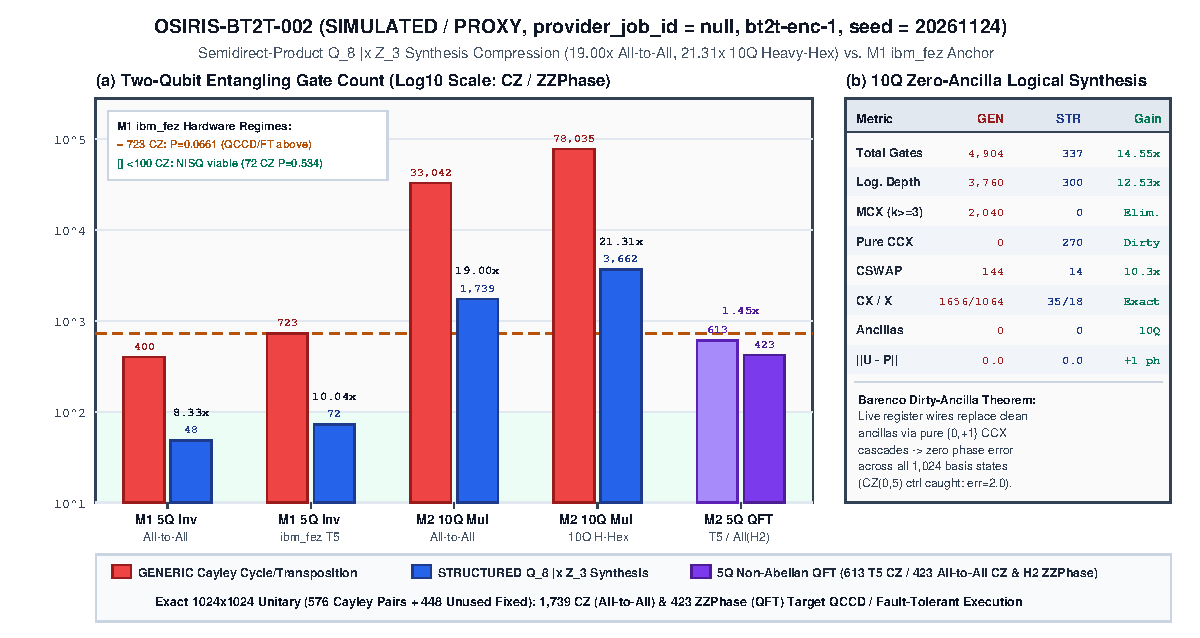
\includegraphics[width=\textwidth]{fig1_bt2t002_semidirect_mul_compression.pdf}
  \caption{Cross-milestone entangling-gate compression and $\btmMulQubits$-qubit zero-ancilla logical synthesis under frozen encoding \btmEncVer\ (\btmExperimentId, \btmExecTier\ / \btmProxyTier, \texttt{provider\_job\_id:} \btmJobId, seed $\btmSeed$). (a)~Log-scale comparison of generic Cayley cycle/transposition synthesis versus structured $Q_8 \rtimes \mathbb{Z}_3$ synthesis across Milestone~1 ($\btmRegQubits$-qubit inversion: \btmMoneAtaRatio\ all-to-all, \btmMoneFezRatio\ on \btmMoneBackend\ job \btmMoneJobId) and Milestone~2 ($\btmMulQubits$-qubit multiplication: \btmMulAtaCzRatio\ all-to-all from $\btmMulAtaGenCz$ to $\btmMulAtaStructCz$ \texttt{CZ}, and \btmMulHhCzRatio\ on $\btmMulQubits$-qubit heavy-hex from $\btmMulHhGenCz$ to $\btmMulHhStructCz$ \texttt{CZ}), alongside the $\btmRegQubits$-qubit non-abelian $2T$ QFT ($\btmQftTfCz$ \texttt{T5} \texttt{CZ} / $\btmQftAtaCz$ all-to-all \texttt{CZ} and \texttt{H2} \texttt{ZZPhase}). (b)~Zero-ancilla logical gate compression ($\btmMulLogGateRatio$ gate reduction, $\btmMulLogDepthRatio$ depth reduction, complete elimination of $\btmMulGenMcx$ $k \ge 3$ \texttt{MCX} gates via Barenco dirty-ancilla \texttt{CCX} cascades).}
  \label{fig:btm_mul_compression}
\end{figure*}

\begin{table*}[t]
\caption{Logical and local \btmProxyTier\ native compilation benchmarks (\texttt{seed\_transpiler} $= \btmSeed$; QASM2 SHA-256 prefixes \btmStructQasmSha, \btmGenQasmSha, and \btmQftQasmSha) for Milestone~2 $\btmMulQubits$-qubit $2T$ multiplication and $\btmRegQubits$-qubit non-abelian $2T$ QFT alongside the Milestone~1 \btmMoneBackend\ hardware anchor (\btmMoneJobId).}
\label{tab:btm_compilation}
\begin{ruledtabular}
\begin{tabular}{llrrrlr}
Primitive \& Compilation Target & Synthesis Arm & Entangling / Key Gates & Total Gates & Depth & Gain / Ratio & Unitary / Tier Verification \\
\hline
\btmTableMulCompilationRows
\end{tabular}
\end{ruledtabular}
\end{table*}

Figure~\ref{fig:btm_mul_compression} and Table~\ref{tab:btm_compilation} summarize local \btmProxyTier\ transpilation onto $\{\mathrm{RZ},\sqrt{X},X,\mathrm{CZ}\}$ at \texttt{optimization\_level=3} (\texttt{seed\_transpiler} $= \btmSeed$). Semidirect synthesis compresses native \texttt{CZ} count by \btmMulAtaCzRatio\ (\btmMulAtaCzRatioFour) on all-to-all connectivity ($\btmMulAtaGenCz \to \btmMulAtaStructCz$ \texttt{CZ}, depth $\btmMulAtaGenDepth \to \btmMulAtaStructDepth$, \btmMulAtaDepthRatio, phase-aligned operator residual $\btmMulAtaStructErr$) and by \btmMulHhCzRatio\ (\btmMulHhCzRatioFour) on the $\btmMulQubits$-qubit heavy-hex graph ($\btmMulHhGenCz \to \btmMulHhStructCz$ \texttt{CZ}, depth $\btmMulHhGenDepth \to \btmMulHhStructDepth$, \btmMulHhDepthRatio, residual $\btmMulHhStructErr$, reducing heavy-hex SWAP expansion from \btmMulHhSwapOverheadGen\ to \btmMulHhSwapOverheadStruct).

\section{Seven-Irrep Peter--Weyl Non-Abelian Quantum Fourier Transform}

\subsection{Complete Unitary Irreps of $2T$ and $\widetilde{F}_{2T} = F_{2T} \oplus I_8$}
The binary tetrahedral group $2T$ partitions into $\btmNumIrreps$ conjugacy classes ($\{+\mathbf{1}\}$, $\{-\mathbf{1}\}$, $\{\pm\mathbf{i},\pm\mathbf{j},\pm\mathbf{k}\}$, and four size-$4$ Hurwitz classes) and therefore admits exactly $\btmNumIrreps$ inequivalent unitary irreducible representations $\rho_\alpha$ whose dimensions $(1,1,1,2,2,2,3)$ satisfy the Plancherel completeness relation
\begin{equation}
  \sum_{\alpha=1}^{\btmNumIrreps} d_\alpha^2 = 1^2 + 1^2 + 1^2 + 2^2 + 2^2 + 2^2 + 3^2 = \btmSumDSquared = |2T|.
  \label{eq:plancherel_dims}
\end{equation}
In \texttt{bt2t\_qft.py} (SHA-256 prefix \btmQftPySha), all $\btmNumIrreps$ irreps are constructed analytically from \btmEncVer\ without numerical eigensolvers:
\begin{enumerate}
  \item \emph{$\btmNumOneDIrreps$ one-dimensional characters $\chi_r$ ($r \in \{0,1,2\}$, $d=1$):} Lifted from the abelianization $2T / Q_8 \cong \mathbb{Z}_3$ via $\chi_r(g) = [\zeta_3^{r c(g)}]$ with $\zeta_3 = e^{2\pi i/3}$ and kernel $Q_8$.
  \item \emph{$\btmNumTwoDIrreps$ two-dimensional spinor irreps $\rho_{2,r}$ ($r \in \{0,1,2\}$, $d=2$):} Faithful unitary representations $\rho_{2,r}(g) = \chi_r(g)\, U_{SU(2)}(g) \in U(2)$, where $U_{SU(2)}(g) = \tfrac{1}{2}(a I_2 - i b \sigma_x - i c \sigma_y - i d \sigma_z)$ maps $-\mathbf{1} \mapsto -I_2$.
  \item \emph{$\btmNumThreeDIrreps$ three-dimensional tetrahedral vector irrep $\rho_3$ ($d=3$):} Real special-orthogonal matrices in $SO(3) \cong 2T / \{\pm\mathbf{1}\} \cong A_4$ defined by the adjoint Pauli action $U_{SU(2)}(g)\,\sigma_a\,U_{SU(2)}(g)^\dagger = \sum_{b=1}^3 [\rho_3(g)]_{b,a}\sigma_b$.
\end{enumerate}

Table~\ref{tab:btm_irreps} reports exhaustive verification across all $\btmGroupOrder$ elements and all $\btmValidPairs$ group pairs: maximum unitarity residual $\|\rho_\alpha(g)\rho_\alpha(g)^\dagger - I_{d_\alpha}\|_\infty \le \btmIrrepUnitMaxErr$, maximum homomorphism residual $\|\rho_\alpha(gh) - \rho_\alpha(g)\rho_\alpha(h)\|_{\max} \le \btmIrrepHomMaxErr$, and character-table Gram orthogonality $\|\tfrac{1}{24} X X^\dagger - I_7\|_\infty = \btmCharOrthErr$.

\begin{table*}[t]
\caption{Complete $\btmNumIrreps$-irrep Peter--Weyl decomposition of $2T$ under frozen encoding \btmEncVer\ ($\sum_\alpha d_\alpha^2 = \btmSumDSquared$; character Gram orthogonality residual $\btmCharOrthErr$; $32\times 32$ unitary residual $\|\widetilde{F}_{2T}\widetilde{F}_{2T}^\dagger - I_{32}\|_\infty = \btmQftUnitarityErr$).}
\label{tab:btm_irreps}
\begin{ruledtabular}
\begin{tabular}{lrrlrrrl}
Irrep $\alpha$ & $d_\alpha$ & Sector $d_\alpha^2$ & Row Slice (Blocks) & Schur RMS $d_\alpha^{-1/2}$ & Max Unitarity Err & $\btmValidPairs$-Pair Hom.\ Err & Analytic Construction \\
\hline
\btmTableIrrepPeterWeylRows
\end{tabular}
\end{ruledtabular}
\end{table*}

Assembling the $24\times 24$ Peter--Weyl Fourier matrix with row index $(\alpha, k, j)$ ordered by irrep $\alpha$, outer multiplicity $k \in \{0,\dots,d_\alpha - 1\}$, and inner representation row $j \in \{0,\dots,d_\alpha - 1\}$,
\begin{equation}
  \bigl[F_{2T}\bigr]_{(\alpha,k,j),\, g} = \sqrt{\frac{d_\alpha}{24}}\,\bigl[\rho_\alpha(g)\bigr]_{j,k}, \qquad
  \widetilde{F}_{2T} = F_{2T} \oplus I_8,
  \label{eq:peter_weyl_qft}
\end{equation}
yields an exact $\btmRegQubits$-qubit unitary on $\mathbb{C}^{32}$ ($\|\widetilde{F}_{2T}\widetilde{F}_{2T}^\dagger - I_{32}\|_\infty = \btmQftUnitarityErr$, unused-codeword identity error $\btmQftUnusedIdErr$) via Schur's matrix-element orthogonality relations. Under $(k,j)$ row ordering, $F_{2T}$ simultaneously block-diagonalizes every left translation $L_g|x\rangle = |gx\rangle$ and right translation $R_g|x\rangle = |xg^{-1}\rangle$ ($g \in 2T$):
\begin{equation}
  F_{2T} L_g F_{2T}^\dagger = \bigoplus_{\alpha} \bigl(I_{d_\alpha} \otimes \rho_\alpha(g)\bigr), \quad
  F_{2T} R_g F_{2T}^\dagger = \bigoplus_{\alpha} \bigl(\overline{\rho_\alpha(g)} \otimes I_{d_\alpha}\bigr),
  \label{eq:block_diag}
\end{equation}
partitioning $F_{2T} L_g F_{2T}^\dagger$ into $\btmNumContigBlocks$ contiguous diagonal blocks of sizes $\btmBlockSizesStr$ ($\btmDiagBlockEntries$ on-block entries with exact Schur root-mean-square magnitudes $d_\alpha^{-1/2} \in \{\btmRmsOneD, \btmRmsTwoD, \btmRmsThreeD\}$, and $\btmOffBlockEntries$ off-block entries bounded by $\btmLeftOffBlockErr$; on-block residual $\btmLeftOnBlockErr$; right-regular off-sector residual $\btmRightOffIrrepErr$ and on-block residual $\btmRightOnBlockErr$). On seeded complex functions $a, b : 2T \to \mathbb{C}$, Plancherel norm preservation holds to $\btmPlancherelErr$ and the non-abelian convolution identity $\widehat{a * b}(\alpha) = \widehat{a}(\alpha)\widehat{b}(\alpha)$ holds to $\btmConvMaxErr$. Synthesizing $\widetilde{F}_{2T}$ on $\btmRegQubits$ qubits via Quantum Shannon Decomposition produces $\btmQftLogCx$ \texttt{CX}, $\btmQftLogU$ $U$, $\btmQftLogRz$ $R_z$, and $\btmQftLogH$ $H$ gates ($\btmQftLogTotal$ logical gates, depth $\btmQftLogDepth$, $\|U_{\mathrm{QSD}} - \widetilde{F}_{2T}\|_{\max} = \btmQftDirectOpErr$), compiling under \btmProxyTier\ ISA targets to $\btmQftAtaCz$ \texttt{CZ} all-to-all (depth $\btmQftAtaDepth$; opt~1 depth $\btmQftAtaOptOneDepth$), $\btmQftTfCz$ \texttt{CZ} on heavy-hex \texttt{T5} (depth $\btmQftTfDepth$, a \btmQftTfOverhead\ routing factor; opt~1 $\btmQftTfOptOneCz$ \texttt{CZ}), and $\btmQftTkZz$ \texttt{ZZPhase} on \texttt{pytket} \texttt{H2} (depth $\btmQftTkDepth$, error $\btmQftTkErr$).

\section{Non-Abelian Hidden Subgroup Coset Tomography and Hardware Feasibility}

\begin{figure*}[t]
  \centering
  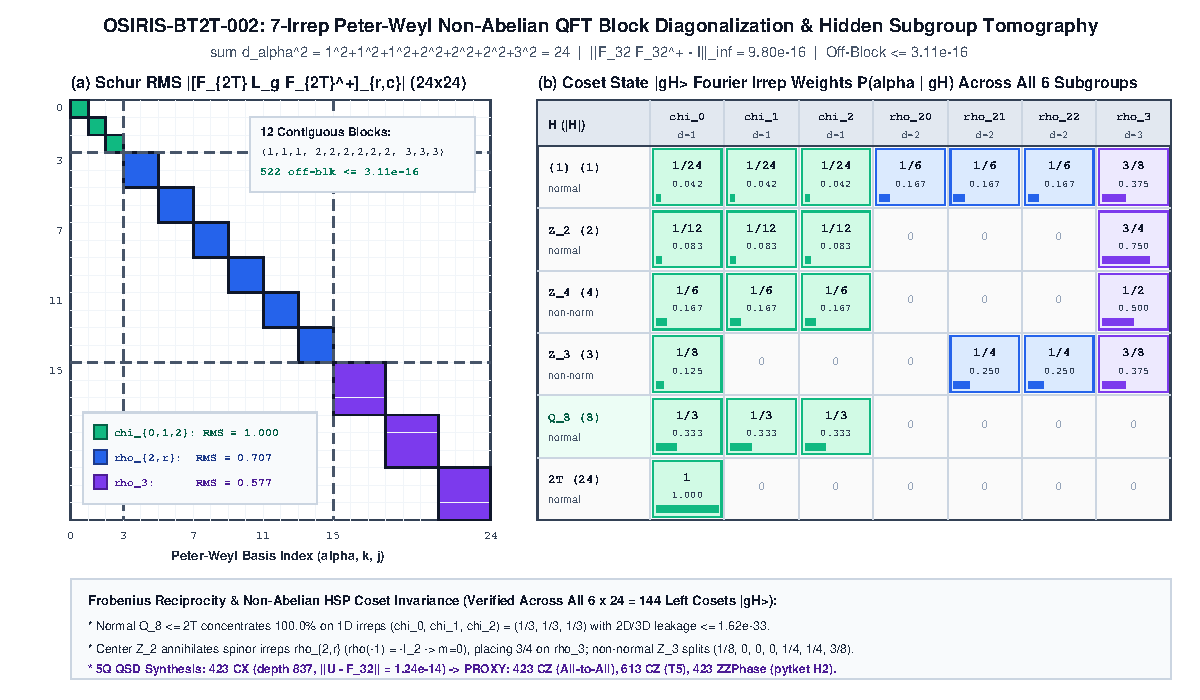
\includegraphics[width=\textwidth]{fig2_bt2t002_peter_weyl_qft_and_hsp.pdf}
  \caption{Peter--Weyl block-diagonalization and Hidden Subgroup coset-state tomography over $2T$ (\btmExperimentId, \btmExecTier). (a)~Exact $24\times 24$ Schur RMS amplitude matrix $\bigl(\tfrac{1}{24}\sum_{g \in 2T}|[F_{2T}L_g F_{2T}^\dagger]_{r,c}|^2\bigr)^{1/2}$ isolating the $\btmNumContigBlocks$ contiguous diagonal blocks $\btmBlockSizesStr$ ($\btmDiagBlockEntries$ active entries with RMS $d_\alpha^{-1/2} \in \{\btmRmsOneD, \btmRmsTwoD, \btmRmsThreeD\}$; all $\btmOffBlockEntries$ off-block entries $\le \btmLeftOffBlockErr$). (b)~Measured Fourier irrep-sector probability distributions $P(\alpha \mid gH)$ across all $\btmNumSubgroups$ canonical subgroups $H \le 2T$ (verified across all $\btmTotalCosetTests$ left cosets with error $\le \btmHspMaxWeightErrAll$, forbidden leakage $\le \btmHspMaxForbLeakAll$, and $\btmHspMaxUnusedLeakAll$ unused-codeword leakage).}
  \label{fig:btm_qft_hsp}
\end{figure*}

\begin{table*}[t]
\caption{Exact non-abelian HSP Fourier irrep-sector distributions $P(\alpha \mid gH) = d_\alpha |H| m_\alpha(H)/24$ verified across all $\btmGroupOrder$ left cosets $|gH\rangle$ of all $\btmNumSubgroups$ canonical subgroups $H \le 2T$ ($\btmTotalCosetTests$ coset states; unused-$8$ leakage identically $\btmHspMaxUnusedLeakAll$).}
\label{tab:btm_hsp}
\begin{ruledtabular}
\begin{tabular}{lrcrrrrrrrrrr}
Subgroup $H$ & $|H|$ & Normal & $m_\alpha(H)$ & $\chi_0$ & $\chi_1$ & $\chi_2$ & $\rho_{2,0}$ & $\rho_{2,1}$ & $\rho_{2,2}$ & $\rho_3$ & Max Coset Err & Forbidden Leak \\
\hline
\btmTableHspSubgroupRows
\end{tabular}
\end{ruledtabular}
\end{table*}

In the standard method for the non-abelian HSP~\cite{MooreRockmoreRussell2006,EttingerHoyerKnill2004}, querying an $H$-periodic oracle prepares a random left coset state $|gH\rangle = |H|^{-1/2}\sum_{h \in H}|gh\rangle$ ($g \in 2T$) in the five-qubit group register. Because $\widetilde{F}_{2T}|gH\rangle = (\bigoplus_\alpha (I_{d_\alpha} \otimes \rho_\alpha(g)))\widetilde{F}_{2T}|H\rangle$ applies local unitary rotations $\rho_\alpha(g)$ purely inside the row space $j$ of each irrep $\alpha$, the total measurement probability on irrep sector $\alpha$ (weak Fourier sampling) is strictly invariant under left coset shift $g \in 2T$ and given by Frobenius reciprocity:
\begin{equation}
  m_\alpha(H) = \frac{1}{|H|}\sum_{h \in H}\chi_\alpha(h), \qquad
  P(\alpha \mid gH) = \frac{d_\alpha\,|H|\,m_\alpha(H)}{24}.
  \label{eq:frobenius_hsp}
\end{equation}

Figure~\ref{fig:btm_qft_hsp}b and Table~\ref{tab:btm_hsp} verify Eq.~\eqref{eq:frobenius_hsp} across all $\btmGroupOrder$ coset shifts of all $\btmNumSubgroups$ canonical subgroups ($\btmTotalCosetTests$ total states, maximum sector-weight deviation $\btmHspMaxWeightErrAll$, unused-$8$ leakage $\btmHspMaxUnusedLeakAll$):
\begin{itemize}
  \item \emph{Normal quaternion subgroup $Q_8 \triangleleft 2T$ ($|H|=\btmQeightOrder$):} Concentrates $\btmQeightOneDWeight$ ($100\%$) of Fourier probability equally across the three one-dimensional irreps $(\chi_0,\chi_1,\chi_2) = (\tfrac{1}{3},\tfrac{1}{3},\tfrac{1}{3}) \approx (\btmQeightEachOneD,\btmQeightEachOneD,\btmQeightEachOneD)$, suppressing leakage into $\rho_{2,r}$ and $\rho_3$ to $\le \btmQeightMaxForbLeak$ ($\btmQeightIdentityLeak$ on $|e Q_8\rangle$).
  \item \emph{Center $\mathbb{Z}_2 = \{\pm\mathbf{1}\}$ ($|H|=2$) and cyclic $\mathbb{Z}_4 = \langle\mathbf{i}\rangle$ ($|H|=4$):} Because $\rho_{2,r}(-\mathbf{1}) = -I_2$, central projection $\tfrac{1}{2}(I_2 + \rho_{2,r}(-\mathbf{1})) = 0$ annihilates all three spinor irreps ($m_{\rho_{2,r}} = 0$), placing $\tfrac{3}{4} = \btmZtwoRhoThreeW$ on $\rho_3$ ($\tfrac{1}{12} \approx \btmZtwoChiW$ on each $\chi_r$) for $\mathbb{Z}_2$ and $\tfrac{1}{2} = \btmZfourRhoThreeW$ on $\rho_3$ ($\tfrac{1}{6} \approx \btmZfourChiW$ on each $\chi_r$) for $\mathbb{Z}_4$.
  \item \emph{Non-normal tetrahedral axis $\mathbb{Z}_3 = \langle\omega\rangle$ ($|H|=\btmZthreeOrder$):} Concentrates onto $(\chi_0, \rho_{2,1}, \rho_{2,2}, \rho_3) = (\tfrac{1}{8}, \tfrac{1}{4}, \tfrac{1}{4}, \tfrac{3}{8}) = (\btmZthreeChiZeroW, \btmZthreeRhoTwoW, \btmZthreeRhoTwoW, \btmZthreeRhoThreeW)$ with $\btmZthreeMaxForbLeak$ forbidden leakage. Because character values $\chi_\alpha$ are class functions, all four conjugate $\mathbb{Z}_3$ subgroups produce identical weak irrep weights, demonstrating concretely why resolving conjugate non-normal subgroups requires strong Fourier measurements across $(j,k)$ basis rows inside $\rho_{2,r}$ and $\rho_3$.
  \item \emph{Extremal subgroups $\{\mathbf{1}\}$ and $2T$:} Yield the Plancherel measure $d_\alpha^2/24 = (\btmTrivChiW, \btmTrivChiW, \btmTrivChiW, \btmTrivRhoTwoW, \btmTrivRhoTwoW, \btmTrivRhoTwoW, \btmTrivRhoThreeW)$ and pure trivial-character support $P(\chi_0 \mid 2T) = \btmFullChiZeroW$ (leakage $\btmFullMaxForbLeak$), respectively.
\end{itemize}

\begin{table*}[t]
\caption{Analytical two-qubit survival envelopes $S = (1 - \epsilon_{2\mathrm{Q}})^{N_{2\mathrm{Q}}}$ across heavy-hex superconducting NISQ ($\epsilon_{2\mathrm{Q}} = \btmEpsHeavyHex$, calibrated to Milestone~1 \btmMoneBackend\ job \btmMoneJobId), current all-to-all trapped-ion QCCD ($\epsilon_{2\mathrm{Q}} = \btmEpsQccd$), and next-generation QCCD / early fault-tolerant logical execution ($\epsilon_{2\mathrm{Q}} = \btmEpsNextGen$).}
\label{tab:btm_feasibility}
\begin{ruledtabular}
\begin{tabular}{lrrrrl}
Group Primitive \& Synthesis & Native 2Q Count (H-Hex / All-to-All) & Heavy-Hex ($\epsilon_{2\mathrm{Q}} = \btmEpsHeavyHex$) & QCCD \texttt{H2} ($\epsilon_{2\mathrm{Q}} = \btmEpsQccd$) & Next-Gen / FT ($\epsilon_{2\mathrm{Q}} = \btmEpsNextGen$) & Architectural Regime \\
\hline
\btmTableFeasibilityRows
\end{tabular}
\end{ruledtabular}
\end{table*}

Finally, Table~\ref{tab:btm_feasibility} connects our exact \btmProxyTier\ gate counts to physical QPU execution via the analytical survival envelope $S(\epsilon_{2\mathrm{Q}}, N_{2\mathrm{Q}}) = (1 - \epsilon_{2\mathrm{Q}})^{N_{2\mathrm{Q}}}$ anchored to Milestone~1 hardware data on \btmMoneBackend~\cite{DavisBT2T001Fez2026}. On heavy-hex transmons ($\epsilon_{2\mathrm{Q}} \approx \btmEpsHeavyHex$ effective per-\texttt{CZ} error including routing idle decoherence, where $\btmMoneFezStructCz$ \texttt{CZ} yielded $S = \btmSurvHhMoneStruct$ versus $\btmMonePValidStructMit$ readout-mitigated and $\btmMoneFezGenCz$ \texttt{CZ} yielded $S = \btmSurvHhMoneGen$ versus $\btmMonePValidGenMit$), the $\btmRegQubits$-qubit $2T$ QFT ($\btmQftTfCz$ \texttt{CZ}, $S \approx \btmSurvHhQft$) and $\btmMulQubits$-qubit $2T$ multiplier ($\btmMulHhStructCz$ \texttt{CZ}, $S \approx \btmSurvHhMulStruct$) lie beyond unmitigated heavy-hex NISQ coherence---justifying our governance decision not to expend superconducting QPU quota on unmitigated Milestone~2 circuits (\texttt{provider\_job\_id:} \btmJobId, \btmQpuSec\,s QPU). Conversely, on all-to-all QCCD trapped-ion processors ($\epsilon_{2\mathrm{Q}} \approx \btmEpsQccd$), eliminating heavy-hex SWAP overhead yields $S \approx \btmSurvQccdQft$ for the $\btmQftTkZz$-\texttt{ZZPhase} non-abelian QFT (immediately viable for coherent HSP coset tomography) and $S \approx \btmSurvQccdMulStruct$ for $\btmMulAtaStructCz$-gate $2T$ multiplication (well above the $1/1024 \approx \btmTenQRandFloor$ random floor, whereas generic $\btmMulAtaGenCz$-gate synthesis collapses to $\btmSurvQccdMulGen$), rising to $\btmSurvFtQft$ and $\btmSurvFtMulStruct$ at $\epsilon_{2\mathrm{Q}} = \btmEpsNextGen$ on next-generation QCCD and early fault-tolerant logical registers.

\section{Conclusion}
Semidirect-product synthesis over $2T \cong Q_8 \rtimes \mathbb{Z}_3$ combined with $\mathbb{F}_2$ M\"obius unused-sector gating and Barenco dirty-ancilla \texttt{CCX} live-wire invariance compresses $\btmMulQubits$-qubit zero-ancilla reversible $2T$ multiplication by \btmMulAtaCzRatio\ all-to-all ($\btmMulAtaStructCz$ versus $\btmMulAtaGenCz$ \texttt{CZ}) and \btmMulHhCzRatio\ on heavy-hex ($\btmMulHhStructCz$ versus $\btmMulHhGenCz$ \texttt{CZ}) with exact $1024\times 1024$ complex unitary fidelity, while our analytic $\btmNumIrreps$-irrep Peter--Weyl $\btmRegQubits$-qubit QFT ($\btmQftAtaCz$ all-to-all \texttt{CZ} / $\btmQftTkZz$ \texttt{H2} \texttt{ZZPhase}) simultaneously block-diagonalizes all $\btmGroupOrder$ group translations and resolves all $\btmNumSubgroups$ canonical subgroups of $2T$. Paired with Milestone~1 hardware attestation on \btmMoneBackend, all $\btmChecksPassed / \btmChecksTotal$ offline checks pass and establish quantitative gate-count targets for non-abelian gauge-link simulation on all-to-all QCCD and fault-tolerant quantum computers.

\section*{Data and Code Availability}
Audited clean-room modules \texttt{bt2t\_mul.py} (\btmMulPySha), \texttt{bt2t\_qft.py} (\btmQftPySha), \texttt{verify\_bt2t002.py} (\btmVerifyPySha), verification manifest \texttt{manifest\_bt2t002.json} (\btmManifestSha), Milestone~1 hardware anchor (\btmMoneResSha), and the RFC~8785 reproducibility capsule (\btmCapsuleSha) are archived under \texttt{experiments/bt2t\_primitives/} and \texttt{papers/bt2t002\_mul\_and\_nonabelian\_qft/} and locked in \texttt{SHA256SUMS.txt}.

\begin{thebibliography}{9}
\bibitem{LammLawrenceYamauchi2019} H. Lamm, S. Lawrence, and Y. Yamauchi (NuQS Collaboration), Phys. Rev. D \textbf{100}, 034518 (2019).
\bibitem{BenderZoharCirac2018} J. Bender, E. Zohar, A. Farace, and J. I. Cirac, New J. Phys. \textbf{20}, 093001 (2018).
\bibitem{MooreRockmoreRussell2006} C. Moore, D. Rockmore, and A. Russell, ACM Trans. Algorithms \textbf{2}, 707 (2006).
\bibitem{EttingerHoyerKnill2004} M. Ettinger, P. H{\o}yer, and E. Knill, Inf. Process. Lett. \textbf{91}, 43 (2004).
\bibitem{MochxonKitaevPreskill2004} C. Mochon, Phys. Rev. A \textbf{69}, 032306 (2004).
\bibitem{Barenco1995} A. Barenco, C. H. Bennett, R. Cleve, D. P. DiVincenzo, N. Margolus, P. Shor, T. Sleator, J. A. Smolin, and H. Weinfurter, Phys. Rev. A \textbf{52}, 3457 (1995).
\bibitem{DavisBT2T001Fez2026} D. P. Davis, \emph{Exact Binary Tetrahedral Group Inversion on a 5-Qubit Heavy-Hex Superconducting Register: Coset-Parity Synthesis Compression and Unflagged Readout Staleness (\texttt{OSIRIS-BT2T-001-FEZ})}, OSIRIS Archival Preprint (2026).
\bibitem{DavisRO0607Zenodo2026} D. P. Davis, \emph{Transient Readout Staleness and Multiplexed Isolation on 156-Qubit IBM Heron r2 Processors (RO-06/RO-07)}, Zenodo (2026), \texttt{doi:10.5281/zenodo.24420902}.
\end{thebibliography}

\end{document}
